This layer is the heart of the core autonomous functionalities of the Turing Board. We use computer
vision and depth imagery to determine the board’s surroundings and calculate the best path to move
forward. The user will have, strapped around their ankle, an anklet-like contraption consisting of a
pattern of ArUco markers for the Follow Along feature. This layer tracks the movement of the user
through the anklet to determine how to instruct the combination of motors to move so as to follow the
user at an appropriate pace. It is also responsible for detecting possible obstacles when operating on its
own to find the user as part of the Summon feature.
\subsection{Layer Hardware}
The required hardware components include the NVIDIA Jetson TX2 as the main compute module and the Intel RealSense  D432 Depth Camera.

\subsection{Layer Operating System}
The NVIDIA Jetson TX2 is running Ubuntu 18.04. 

\subsection{Layer Software Dependencies}
This layer requires the OpenCV v4.2.2 or higher compiled with cuDNN enabled. A more detailed and exhaustive list can be obtained from. https://github.com/TuringBoard/turing-board-vision/blob/main/Configuring%20the%20NVIDIA%20Jetson%20TX2.md.
% I know the text doesn't wrap to the next line for the link. Latex is stupid. I am not pressed about it. - Sahaj 

\subsection{RGB IMAGERY SUBSYSTEM}
RGB Imagery of the front of the board is used as input in making various position specific calculations pertaining to navigation.

%%%%%%%%%%%%%%%%%%%%%%%%%%%%%%%%%%%%%%%%%%%%%%%%%%%%%%%%%%
%  BE SURE TO UPDATE THE IMAGE CAPTION
\begin{figure}[h!]
	\centering
 	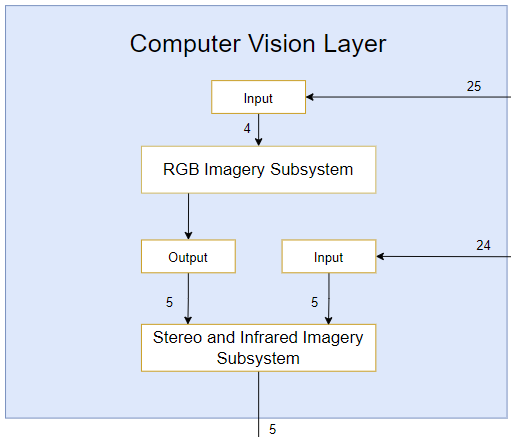
\includegraphics[width=0.60\textwidth]{images/CV.png} % Image
 \caption{CV Layer Subsystem} % Caption
\end{figure}

\subsubsection{Subsystem Hardware}
This subsystem requires the NVIDIA Jetson TX2 and the Intel RealSense  D432 Depth Camera.

\subsubsection{Subsystem Operating System}
Ubuntu 18.04.  

\subsubsection{Subsystem Software Dependencies}
This layer requires the OpenCV v4.2.2 or higher compiled with cuDNN enabled. A more detailed and exhaustive list can be obtained from. https://github.com/TuringBoard/turing-board-vision/blob/main/Configuring%20the%20NVIDIA%20Jetson%20TX2.md.
% I know the text doesn't wrap to the next line for the link. Latex is stupid. I am not pressed about it. - Sahaj 


\subsubsection{Subsystem Programming Languages}
Python 3.x.

\subsubsection{Subsystem Data Structures}
Arrays, HashMaps, Graphs, Trees.

\subsubsection{Subsystem Data Processing}
SIFT, RANSAC, Canny Edge Detection.


